% 
% topic Template for ME3023 - Measurements in Mechanincal Systems - Tennessee Technological University
%
% Spring 2020 - Summer 2020
% Tristan Hill, May 31, 2020
% Module 3 - Calibration
% Topic 1 - Accuracy and Precesion   ->  (4th Topic)
%

%\documentclass{beamer}                         % for presentation (has nav buttons at bottom)
\documentclass[handout]{beamer}  % for handout 
\usepackage{beamerthemesplit}
\usepackage{amsmath}
\usepackage{listings}
\usepackage{multicol}
\usepackage{framed}

\beamertemplateballitem

\definecolor{TTUpurple}{rgb}{0.3098, 0.1607, 0.5176} % TTU Purple (primary)
\definecolor{TTUgold}{rgb}{1.0000, 0.8666, 0.0000} % TTU Gold (primary)

\setbeamercolor{palette primary}{bg=TTUpurple,fg=TTUgold}
\setbeamercolor{palette secondary}{bg=black,fg=TTUgold}
\setbeamercolor{palette tertiary}{bg=black,fg=TTUpurple}
\setbeamercolor{palette quaternary}{bg=TTUgold,fg=black}
\setbeamercolor{structure}{fg=TTUpurple} % itemize, enumerate, etc
\setbeamercolor{section in toc}{fg=TTUpurple} % TOC sections

% custom colors 
\definecolor{mygray}{rgb}{.6, .6, .6}
\definecolor{mypurple}{rgb}{0.6,0.1961,0.8}
\definecolor{mybrown}{rgb}{0.5451,0.2706,0.0745}
\definecolor{mygreen}{rgb}{0, .39, 0}
\definecolor{mypink}{rgb}{0.9960, 0, 0.9960}

% color commands
\newcommand{\R}{\color{red}}
\newcommand{\B}{\color{blue}}
\newcommand{\BR}{\color{mybrown}}
\newcommand{\K}{\color{black}}
\newcommand{\G}{\color{mygreen}}
\newcommand{\PR}{\color{mypurple}}
\newcommand{\PN}{\color{mypink}}
\newcommand{\GD}{\color{TTUgold}}
\newcommand{\OR}{\color{orange}}

\newcommand{\Lagr}{\mathcal{L}} % lagrangian

\newcommand{\hspcu}{\underline{\hspace{25mm}}} % large horizontal space w underline

\newcommand{\vspccc}{\vspace{6mm}\\} % large vertical space
\newcommand{\vspcc}{\vspace{4mm}\\}   % medium vertical space
\newcommand{\vspc}{\vspace{2mm}\\}     % small vertical space

\newcommand{\hspcccc}{\hspace{10mm}} % large horizontal space
\newcommand{\hspccc}{\hspace{6mm}} % large horizontal space
\newcommand{\hspcc}{\hspace{4mm}}   % medium horizontal space
\newcommand{\hspc}{\hspace{2mm}}     % small horizontal space


\author{ME3023 - Measurements in Mechanical Systems} % original formatting from Mike Renfro, September 21, 2004

\newcommand{\MNUM}{3\hspace{2mm}} % Module number
\newcommand{\TNUM}{1\hspace{2mm}} % Topic number  ->  (4th Topic)
\newcommand{\moduletitle}{Calibration }
\newcommand{\topictitle}{ Standards and Units} 

\newcommand{\sectiontitleI}{Thought Experiment Continued}
\newcommand{\sectiontitleII}{Standards and Calibration}
\newcommand{\sectiontitleIII}{Base Dimensions and Unit}
\newcommand{\sectiontitleIV}{Hierarchy of Standards}

\title{Lecture Module - \moduletitle}

\date{Mechanical Engineering\vspc Tennessee Technological University}

\begin{document}

\lstset{language=MATLAB,basicstyle=\ttfamily\small,showstringspaces=false}

\frame{\titlepage \center\begin{framed}\Large \textbf{Topic \TNUM - \topictitle}\end{framed} \vspace{5mm}}

% Section 0: Outline
\frame{

\large \textbf{Topic \TNUM - \topictitle} \vspace{3mm}\\

\begin{itemize}
	\item \sectiontitleI		\vspc % Section I
	\item \sectiontitleII 	\vspc % Section II
	\item \sectiontitleIII 	\vspc %Section III
	\item \sectiontitleIV 	\vspc %Section IV
\end{itemize}

}

% Section I:
\section{\sectiontitleI}

\frame{
\frametitle{\sectiontitleI}

{\bf Thought Experiment}: Look around the room and choose an object. It can be anything. Ask yourself the following questions. \vspc
\begin{itemize}
\item What is the {\bf\G true} length of the object? \vspc
\item What is the physical {\PR meaning} of that number? \vspc
\item What do the {\B units} relate to?
\end{itemize}

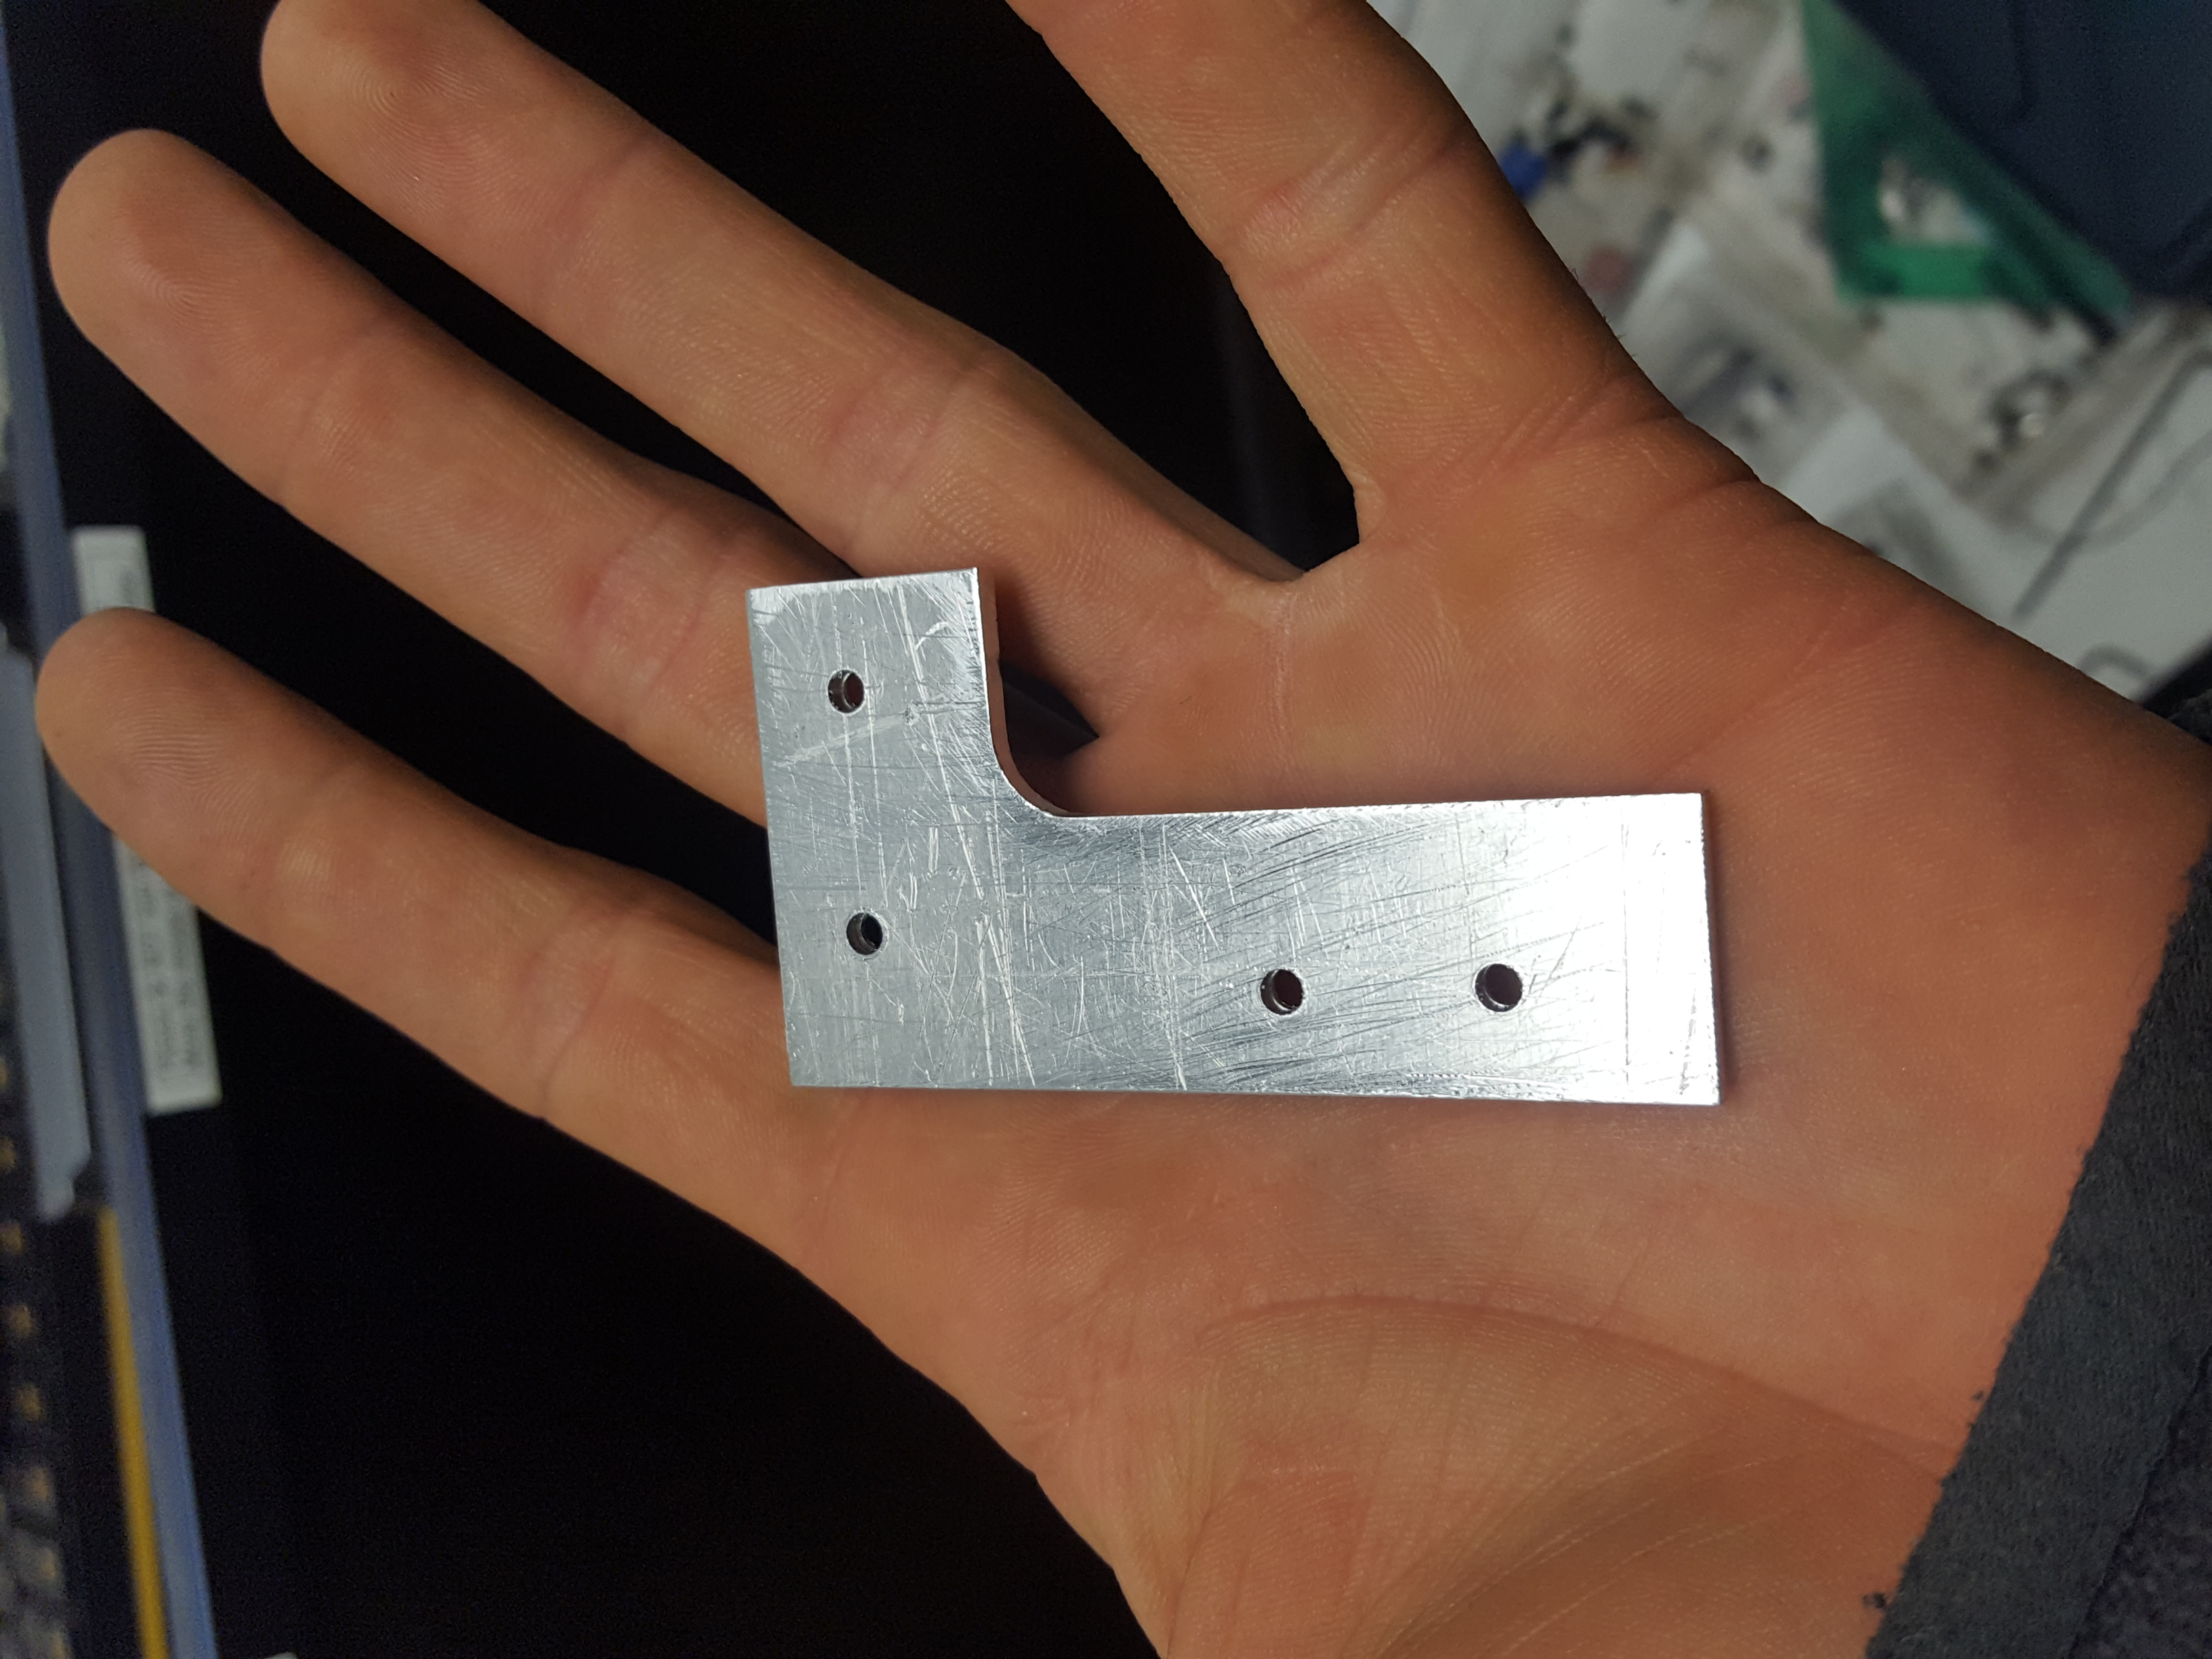
\includegraphics[scale=.025,angle=-90,origin=c]{bracket.jpg}
{\tiny Image: T.Hill}
}


% Section II:
\section{\sectiontitleII}

\frame{
\frametitle{\sectiontitleII}

When a measurement system is \hspcu, its indicated value is compared directly with a {\BR reference
value}. This {\BR  reference value} forms the basis of the comparison and is known as the \hspcu. This
\hspcu may be based on the output from a piece of equipment, from an object having a well-
defined physical attribute to be used as a comparison, or from a well-accepted technique known to
produce a reliable value.\vspace{5mm}\\

{\tiny Text: \underline{Theory and Design of Mechanical Measurements, 5th Edition}}
}

\frame{
\frametitle{\sectiontitleII}

A {\G dimension} \vspace{15mm}\\
A {\PN unit} \vspace{15mm}\\

{\tiny Text: \underline{Theory and Design of Mechanical Measurements, 5th Edition}}

}

% Section III:
\section{\sectiontitleIII}

\frame{
\frametitle{\sectiontitleIII}

The dimension of mass is defined by the kilogram. Originally, the unit of the kilogram was defined
by the mass of one liter of water at room temperature. But today an equivalent yet more consistent
definition defines the kilogram exactly as the mass of a particular platinum-iridium cylindrical bar
that is maintained under very specific conditions at the International Bureau of Weights and
Measures located in \hspcu. This particular bar (\hspcu\hspcu\hspcu\hspcu) forms the primary standard for the kilogram. It remains today as the only basic unit
still defined in terms of a material object.

{\tiny Text: \underline{Theory and Design of Mechanical Measurements, 5th Edition}}
}


\frame{
\frametitle{\sectiontitleIII}

The \hspcu relate directly to a standard (historically).\vspc

\renewcommand{\arraystretch}{1.2}
\begin{tabular}{|c|cc|cc|} \hline
\textbf{Unit}&\textbf{SI}&&\textbf{I-P}&\\ \hline\hline
Length&meter&$(m)$&foot&$(ft)$\\ \hline
Mass&kilogram&$(kg)$&slug&$(slug)$ \\\hline
Time&second&$(s)$&second&$(sec)$\\ \hline
Temperature&degrees&$(^\circ C$, $^\circ K)$&degrees&$(^\circ F$, $^\circ R)$ \\ \hline
Current&ampere&$(A)$&ampere&$(A)$\\ \hline
Substance&mole&$(mol)$&mole&$(mol)$\\ \hline
Light Intensity&candela&$(cd)$&candela&$(cd)$\\ \hline
%force&newton&(N)&pound&(lb)\\ \hline
%energy&joule&(J)&foot-pound&(ft-lb)\\ \hline
%power&watt&(W)&?&(ft-lb/sec)\\ \hline
\end{tabular}

}

\frame{
\frametitle{\sectiontitleIII}

Common \hspcu are defined in terms of \hspcu . \vspc
\renewcommand{\arraystretch}{1.2}
\begin{tabular}{|c|cc|cc|} \hline
\textbf{Unit}&\textbf{SI} &&\textbf{I-P}&\\ \hline\hline
Force&newton&$(N)$&pound-force&$(lb_f)$\\ \hline
Voltage&volt&$(V)$&volt&$(V)$\\ \hline
Resistance&ohm&$(\Omega)$&ohm&$(\Omega)$\\ \hline
Capacitance&farah&$(F)$&farah&$(F)$ \\ \hline 
Inductance&henry&(H)&henry&(H)\\ \hline
Energy&joule&$(J)$&foot-pound&$(ft-lb)$\\ \hline
Power&watt&$(W)$&foot-pound per second&$(ft-lb/sec)$\\ \hline

\end{tabular}

}

% Section IV:
\section{\sectiontitleIV}

\frame{
\frametitle{\sectiontitleIV}

The known value applied to a measurement system during calibration becomes the standard on which the calibration is based. \vspc 
So how do we pick this standard, and how good is it? \vspc
... primary standards are impractical as standards for normal calibration use ... there exists a hierarchy of reference and secondary standards used to duplicate the primary standards. \vspc
\begin{tabular}{|lcl|}\hline\hline
\hspcu standard&---&Maintained as absolute unit standard\\ \hline
\hspcu standard&---&Used to calibrate local standards\\ \hline
\hspcu standard&---&Used to calibrate working standards\\ \hline
\hspcu standard&---&Used to calibrate local instruments\\ \hline 
\end{tabular}

\vspace{2mm}
{\tiny Text: \underline{Theory and Design of Mechanical Measurements, 5th Edition}}
}


\end{document}





